\documentclass[,jou]{apa6}
\usepackage{lmodern}
\usepackage{amssymb,amsmath}
\usepackage{ifxetex,ifluatex}
\usepackage{fixltx2e} % provides \textsubscript
\ifnum 0\ifxetex 1\fi\ifluatex 1\fi=0 % if pdftex
  \usepackage[T1]{fontenc}
  \usepackage[utf8]{inputenc}
\else % if luatex or xelatex
  \ifxetex
    \usepackage{mathspec}
  \else
    \usepackage{fontspec}
  \fi
  \defaultfontfeatures{Ligatures=TeX,Scale=MatchLowercase}
\fi
% use upquote if available, for straight quotes in verbatim environments
\IfFileExists{upquote.sty}{\usepackage{upquote}}{}
% use microtype if available
\IfFileExists{microtype.sty}{%
\usepackage{microtype}
\UseMicrotypeSet[protrusion]{basicmath} % disable protrusion for tt fonts
}{}
\usepackage{hyperref}
\hypersetup{unicode=true,
            pdftitle={How Many Psychologists Use Questionable Research Practices? Estimating the Population Size of Current QRP Users},
            pdfauthor={Nicholas W. Fox, Nathan Honeycutt, \& Lee Jussim},
            pdfkeywords={questionable research practices, QRPs, social networks, population size
estimation},
            pdfborder={0 0 0},
            breaklinks=true}
\urlstyle{same}  % don't use monospace font for urls
\usepackage{graphicx,grffile}
\makeatletter
\def\maxwidth{\ifdim\Gin@nat@width>\linewidth\linewidth\else\Gin@nat@width\fi}
\def\maxheight{\ifdim\Gin@nat@height>\textheight\textheight\else\Gin@nat@height\fi}
\makeatother
% Scale images if necessary, so that they will not overflow the page
% margins by default, and it is still possible to overwrite the defaults
% using explicit options in \includegraphics[width, height, ...]{}
\setkeys{Gin}{width=\maxwidth,height=\maxheight,keepaspectratio}
\IfFileExists{parskip.sty}{%
\usepackage{parskip}
}{% else
\setlength{\parindent}{0pt}
\setlength{\parskip}{6pt plus 2pt minus 1pt}
}
\setlength{\emergencystretch}{3em}  % prevent overfull lines
\providecommand{\tightlist}{%
  \setlength{\itemsep}{0pt}\setlength{\parskip}{0pt}}
\setcounter{secnumdepth}{0}
% Redefines (sub)paragraphs to behave more like sections
\ifx\paragraph\undefined\else
\let\oldparagraph\paragraph
\renewcommand{\paragraph}[1]{\oldparagraph{#1}\mbox{}}
\fi
\ifx\subparagraph\undefined\else
\let\oldsubparagraph\subparagraph
\renewcommand{\subparagraph}[1]{\oldsubparagraph{#1}\mbox{}}
\fi

%%% Use protect on footnotes to avoid problems with footnotes in titles
\let\rmarkdownfootnote\footnote%
\def\footnote{\protect\rmarkdownfootnote}


  \title{How Many Psychologists Use Questionable Research Practices? Estimating
the Population Size of Current QRP Users}
    \author{Nicholas W. Fox\textsuperscript{1}, Nathan Honeycutt\textsuperscript{1},
\& Lee Jussim\textsuperscript{1}}
    \date{}
  
\shorttitle{How Many Psychologists Use QRPs}
\affiliation{
\vspace{0.5cm}
\textsuperscript{1} Rutgers University}
\keywords{questionable research practices, QRPs, social networks, population size estimation\newline\indent Word count: X}
\usepackage{csquotes}
\usepackage{upgreek}
\captionsetup{font=singlespacing,justification=justified}

\usepackage{longtable}
\usepackage{lscape}
\usepackage{multirow}
\usepackage{tabularx}
\usepackage[flushleft]{threeparttable}
\usepackage{threeparttablex}

\newenvironment{lltable}{\begin{landscape}\begin{center}\begin{ThreePartTable}}{\end{ThreePartTable}\end{center}\end{landscape}}

\makeatletter
\newcommand\LastLTentrywidth{1em}
\newlength\longtablewidth
\setlength{\longtablewidth}{1in}
\newcommand{\getlongtablewidth}{\begingroup \ifcsname LT@\roman{LT@tables}\endcsname \global\longtablewidth=0pt \renewcommand{\LT@entry}[2]{\global\advance\longtablewidth by ##2\relax\gdef\LastLTentrywidth{##2}}\@nameuse{LT@\roman{LT@tables}} \fi \endgroup}



\authornote{Department of Psychology, Rutgers University,
Piscataway NJ 08854

Correspondence concerning this article should be addressed to Nicholas
W. Fox, 53 Avenue E, Room 429, Piscataway NJ 08854. E-mail:
\href{mailto:nwf7@psych.rutgers.edu}{\nolinkurl{nwf7@psych.rutgers.edu}}}

\abstract{
Psychology has been in crisis. Over the past 15 years many high-impact
research findings have failed to replicate, calling into question their
validity. Increased methodological and statistical scrutiny has led to
field-wide introspection on how best to produce robust, reproducible,
research. One focus has been on the use of questionable research
practices. Previous estimates of the number of researchers who use
questionable research practices vary widely, from over 60\% to near
10\%. In the current work, the authors produced three estimates of the
number of American psychologists who have used questionable research
practices in the last 12 months, utilizing direct, indirect, and social
network measures of estimation. We estimate up to 24.40\% of American
psychologists have recently used at least one questionable research
practice. These estimates represent the first step in generating
actionable interventions to resolve the current replication crisis and
increase trust in published research.


}

\usepackage{amsthm}
\newtheorem{theorem}{Theorem}[section]
\newtheorem{lemma}{Lemma}[section]
\theoremstyle{definition}
\newtheorem{definition}{Definition}[section]
\newtheorem{corollary}{Corollary}[section]
\newtheorem{proposition}{Proposition}[section]
\theoremstyle{definition}
\newtheorem{example}{Example}[section]
\theoremstyle{definition}
\newtheorem{exercise}{Exercise}[section]
\theoremstyle{remark}
\newtheorem*{remark}{Remark}
\newtheorem*{solution}{Solution}
\begin{document}
\maketitle

It is the researcher's job to generate theories, test hypotheses,
collect and interpret data, interpret results, and to publish findings.
This is all done to learn more about the world and how it works. In the
course of doing science, the researcher has many decisions to make: How
many subjects will I use? How will I operationalize my variables? What
is the population of interest that I am studying? Should certain
collected observations be excluded?

Each decision point is a \enquote{researcher degree of freedom}
(Simmons, Nelson, \& Simonsohn, 2011), with the potential of introducing
error and bias. Since there is a high level of ambiguity in research,
these degrees of freedom can be resolved in different ways. In reviewing
how researchers deal with outlying observations, Simmons et al. (2011)
found different research groups made independent decisions on the best
course of action. When researchers cleaned data and removed participants
that responded \enquote{too fast}, some defined this as 2 standard
deviations below the mean response speed, some defined it as
observations below 200ms, and others removed the fastest 2.5\% of
respondents. None of these definitions are inherently an incorrect
interpretation of \enquote{too fast}, which is the problem: without
clear standards in place, this type of flexible decision making can
change the overall interpretation of a study's results.

There are many \enquote{degrees of freedom} that exploit the gray areas
of acceptable practice (John, Loewenstein, \& Prelec, 2012; Wicherts et
al., 2016), and that may bias research findings. A choice ten have been
collectively called \enquote{questionable research practices} (QRPs) and
are typically defined as behaviors during data collection, analysis, and
reporting that have the potential to increase false-positive findings in
the literature. While there are many examples of other behaviors that
could be considered questionable, these 10 stand out as being familiar
to most researchers and have been investigated previously (Agnoli,
Wicherts, Veldkamp, Albiero, \& Cubelli, 2017; Fiedler \& Schwarz, 2016;
John et al., 2012). For this study, nine of the ten QRPs were considered
(Table\textasciitilde{}\ref{tab:QRPs}). We did not include
\enquote{fabricated data} (QRP-10) as a questionable research practice
as the authors do not consider this questionable, but fraudulent.

Part of the difficulty with questionable research practices is that
they're questionable: using them is not always a bad thing to do. In
some cases, using these behaviors in science is the correct thing to do.
For example, hypothesizing after the results are known, or HARKing (Item
8 in Table\textasciitilde{}\ref{tab:QRPs}), is the practice of analyzing
data and then changing the original hypothesis to fit with the observed
findings. Generally, this goes against the scientific method of making a
prediction, collecting data, and deciding whether that data supports the
a priori prediction. However, in multi-study research papers, it makes
sense to use the results from earlier studies to inform the hypothesis
of later studies. If hypotheses are changed before the next set of data
is collected, then this is not questionable. This is thoughtfully using
observations to inform future work, the kind of research held in high
regard (Tukey, 1970).

Although there are some instances when QRP use may be justified, most of
times they are used, they are contributing to the false-positive rate
seen in the published literature (Banks et al., 2016; Fanelli, 2009).
Not only can QRP use increase the number of false-positive findings
(e.g., taking a \enquote{non-significant} result and pushing it over a
threshold into being \enquote{significant}), but using multiple QRPs can
also influence the reported effect size of a given finding due to
sampling bias and low power (Button et al., 2013). This can lead to
interpretations that are not warranted by the data.

\subsection{Prevalence of questionable research
practices}\label{prevalence-of-questionable-research-practices}

Consider one of the most basic questions to ask about the replication
crisis: How many people are contributing to it? John et al. (2012) found
63\% of psychologists admitted to publishing work without all the
dependent measure included (at some point in their academic career). As
articulated by Simmons et al. (2011), this is highly problematic because
increasing the number of dependent variables is correlated with an
increase in the probability of finding a significant result. Without
reporting all dependent measures, readers are left with a false
impression of the rarity or truthfulness of the reported findings. But,
this estimate from John et al. (2012) was contested by Fiedler and
Schwarz (2016). In their conceptual replication that used differently
worded questions, a different conceptualization of \enquote{prevalence},
and tested a German (as opposed to an American) cohort of psychologists,
Fiedler and Schwarz (2016) found less than 10\% prevalence of the same
questionable practice (omitting dependent variables).Further
complicating these estimates, Agnoli et al. (2017) recently replicated
the original John et al. (2012) study in an Italian cohort of
psychologists, and found similarly high levels of QRP use (47.9\% of
respondents had omitted dependent variables). There is currently no
consensus on the prevalence of QRPs in psychology, nor any indication of
how these may be related to the current replication crisis in the field.

Given the inconsistencies in assessing the prevalence of QRPs, the
current work sought to expand on the existing literature in two ways.
First, we investigated current QRP use, operationalized as using at
least one of nine QRPs \enquote{in the past 12 months}. This puts QRP
use into the frame of the current replication crisis. Second, we
generated an estimate of QRP use utilizing the social networks of
psychologists. This indirect method, called the generalized network
scale up estimator (GNSUM) (Jing, Qu, Yu, Wang, \& Cui, 2014; M. J.
Salganik et al., 2011; Zhang et al., 2010; Zheng, Salganik, \& Gelman,
2006), used network information from the general population of
psychologists to make size estimates about specific populations existing
within. By tapping into the ego networks of participants (Lu, Roberts,
Lio, Dunbar, \& Crowcroft, 2009), the GNSUM can collect large amounts of
data about population members per participant. Additionally, this method
did not require participants to identify with a potentially stigmatized
group, potentially reducing response bias compared to more traditional
direct estimates.

While network scale up estimators were expected to provide insights into
QRP use prevalence, they have yet to be used in psychology. The authors
assessed the viability of the generalized network scale up estimate in
this context, while also estimating QRP use prevalence using more
traditional methods - namely, a direct estimate, and the unmatched count
technique (UCT). Thus, this work produced three estimates of QRP use
prevalence.

\section{METHOD}\label{method}

The work detailed in this manuscript was preregistered on May 15th,
2017. The preregistration can be found at DOI 10.17605/OSF.IO/XU25N and
www.osf.io/xu25n.

\subsection{Sample}\label{sample}

The frame population was tenured or tenure-track psychologists
associated with a PhD-granting institution in the United States. The
population contained 7,101 individuals as of June 2017. All 7,101
members of this population were contacted via email and asked to
participate. Of the 7,101 email invitations sent, 214 emails bounced
(3.01\%). We collected 613 full responses (8.63\% full response rate),
and 296 partial responses. Only full responses are used in the following
estimations. Additionally, 26 participant responses were removed for
either being marked complete erroneously or due to breaking
estimate-specific criteria. There was no compensation offered for
participantion, and participants had 7 days to complete the survey after
starting. 299 (48.78\%) participants identified as female, 279 (45.51\%)
identified as male, and 19 (3.10\%) chose not to identify their gender.
131 (21.37\%) participants identified as an Assistant Professor, 141
(23.00\%) as Associate Professor, and 208 (33.93\%) as Full Professor.
113 participants identified as tenure or tenure-track, but did not
disclose their tenure level.

\subsection{Data Sources}\label{data-sources}

Data was collected using three surveys (as opposed to the two proposed
in the preregistration), designed and distributed using Qualtrics survey
software (CITATION). Each survey asked questions designed to estimate
the total social network size of the participant, as well as demographic
questions. Surveys 1 and 2 each contained questions appropriate for the
UCT. Survey 3 contained our direct estimate measure and questions used
to determine transmission of QRP-identity information within an
individual's social network.

All surveys included the definition of \enquote{Questionable Research
Practices (QRPs)}. This definition included the list of behaviors
previously defined in the literature as QRPs (see Table), but omitting
\enquote{fabricating data} for reasons addressed earlier. The definition
of QRP was made available on each relevant question with a mouse
rollover that was first demonstrated with the initial definition.

Additionally, QRP use is temporally isolated to \enquote{in the past 12
months}. Although some have found instances of underreporting when using
a 12 month recall (CITATIONS), this time frame is used frequently to
measure current behavior in major national data collection surveys such
as the National Health Interview Survey (NHIS) (CITATION) and the
National Survey on Drug Use and Health (CITATION).

As data was collected between September 2017 and December 2017,
questions framed using \enquote{in the past 12 months} constrains actual
QRP use between September 2016 and December 2017, a time frame of 15
months. Therefore, estimates of current QRP use are based on the number
of psychologists who have used at least one QRP in this time frame.

\subsection{Measures}\label{measures}

\subsubsection{Direct Estimate}\label{direct-estimate}

For comparison to the generalized network scale-up (GNSUM) and unmatched
count technique (UCT) estimates, we estimated the number of QRP users by
direct estimation. This involveds asking members of the target
population whether they have used at least one QRP in the past 12
months, and is calculated as follows:

\begin{equation}
\rho = \frac{c}{n}
\end{equation}

where \(\rho\) is the proportion estimate of people who have used at
least one QRP in the past 12 months, \(c\) is the number of participants
indicating they have used a QRP in the past 12 months, and \(n\) is the
total number of participant responses.

\subsubsection{Unmatched Count
Technique}\label{unmatched-count-technique}

The unmatched count technique is an indirect way of measuring the base
rates of concealable and potentially stigmatized identities {[}Wolter
and Laier (2014);Gervais and Najle (2017)). In this estimate, two groups
of participants are given a list of innocuous items that could apply to
them (e.g., I own a dishwasher; I exercise regularly). The list of items
for both groups is the same except for one additional item that one
group receives and the other does not. This extra item asks about the
concealable identity (e.g., I own a dishwasher; I exercise regularly; I
smoke crack cocaine {[}examples from (Gervais \& Najle, 2017){]}). See
Table\textasciitilde{}\ref{tab:unmatched} for the full list of items
used. Participants are asked to count and report the number of items in
the list that apply to them. At no point does a participant identify
themselves with any particular list item, only the total number of
applicable items. The proportion of participants that identify with the
stigmatized identity is calculated as:

\begin{equation}
\rho = \frac{\sum x_y^s}{n^s} - \frac{\sum x_y^i}{n^i}
\end{equation}

where \(\rho\) is the proportion estimate of people who have used at
least one QRP in the past 12 months, \(x_y^s\) is the number of reported
items for participant \(y\) in the stigma list group \(s\), \(n^s\) is
the total number of participant responses in group \(s\), \(x_y^i\) is
the number of reported items for participant \(y\) in the innocuous list
group \(i\), and \(n^i\) is the total number of participants in group
\(i\).

\subsubsection{Network Scale-Up and Generalized Network Scale-Up
Methods}\label{network-scale-up-and-generalized-network-scale-up-methods}

Network scale-up methods estimate population sizes using information
about the personal networks (i.e., ego networks) of respondents, based
on the assumption that personal networks are, on average, representative
of the population (M. J. Salganik et al., 2011). Participants were asked
about how many people they \enquote{know} in the frame population. In
this study, \enquote{know} was defined as: they know you by face or by
name, you know them by face or by name, you could contact the person if
you wanted to, and you've been in contact in the past two years (Bernard
et al., 2010). Participants were then asked a series of questions to
estimate the total size of their social network, and the number of
people they know who have used at least one QRP in the past 12 months.
Together, the network scale-up can be used to estimate the proportion of
QRP users, and was calculated as follows:

\begin{equation}
\rho = \frac{\sum y_i}{\sum d_i}
\end{equation}

where \(\rho\) is the proportion estimate of people who have used at
least one QRP in the past 12 months, \(y_i\) is the number of people
known in the target group \(y\) by participant \(i\), and \(d_i\) is the
estimated total number of people known \(d\) by participant \(i\) within
the frame population.

Equation 3 makes two assumptions: that members of the general frame
population know all identity information about all members of their ego
networks, and that QRP users have the same size social networks as the
general frame population. Since QRP use is concealable and potentially
stigmatizing, these assumptions may not hold. For that reason, data was
collected from self-identifying QRP users to estimate how QRP-use
identity information transmits through ego networks (tau, \(\tau\), also
called the transmission rate). This data was collected using the game of
contacts method (Salganik2012). A popularity ratio (delta, \(\delta\))
was calculated by dividing the average network size of QRP users by the
average network size of the general frame population.

Together, \(\tau\) and \(\delta\) adjust the network scale-up estimate
in equation 3 into the generalized network scale-up as follows:

\begin{equation}
\rho = \frac{\sum y_i}{\sum d_i} * \frac{1}{\tau} * \frac{1}{\delta}
\end{equation}

where \(\rho\) is the proportion estimate of people who have used at
least one QRP in the past 12 months, \(\frac{\sum y_i}{\sum d_i}\) is
the network scale-up estimate (equation 3), \(\tau\) is the transmission
rate, and \(\delta\) is the popularity ratio. All network scale-up
results are calculated using Equation 4, incorporating \(\tau\) and
\(\delta\).

\subsubsection{Game of Contacts}\label{game-of-contacts}

To estimate the QRP identity transmission rate, \(\tau\), we performed
the game of contacts with participants who self-identified as using at
least one QRP in the past 12 months. For a full description of the game
of contacts, see Salganik et al (2012)). Briefly, this method has
participants (called egos in network terminology) answer a set of
questions about what they know about the QRP use of several others
(called alters) in their social network, and what those alters know
about the participant's QRP use. The questions are semi-graphical and
responses are recorded on a digital 2x2 grid, representing the four
possible ways information can flow through a given ego-alter
relationship. The transmission rate is then calculated as:

\begin{equation}
\tau = \frac{\sum{w_i}}{\sum{x_i}}
\end{equation}

where \(w_i\) is the number of alters that know the ego is a member of
the target population, and \(x_i\) is the total number of alters
generated by the ego. This produced a value between 0 and 1.

This study utilized a digital distribution of the game of contacts. This
method is typically performed in a face-to-face interview setting with
the participant (Salganik2012b). Due to the distributed nature of our
frame population, this was not feasible. Instead, participants were
presented with the game of contacts via Qualtrics. These questions were
pretested with several academics not within the frame population. A
comparison between an in-person and digital game of contacts has been
pre-registered by the authors (GET PREREG LINK) for future study.

\section{Results}\label{results}

The three estimates of recent QRP use in the frame population of
American tenured or tenure-track faculty are summarized in Figure 1, and
described in detail below.

\begin{figure}
\centering
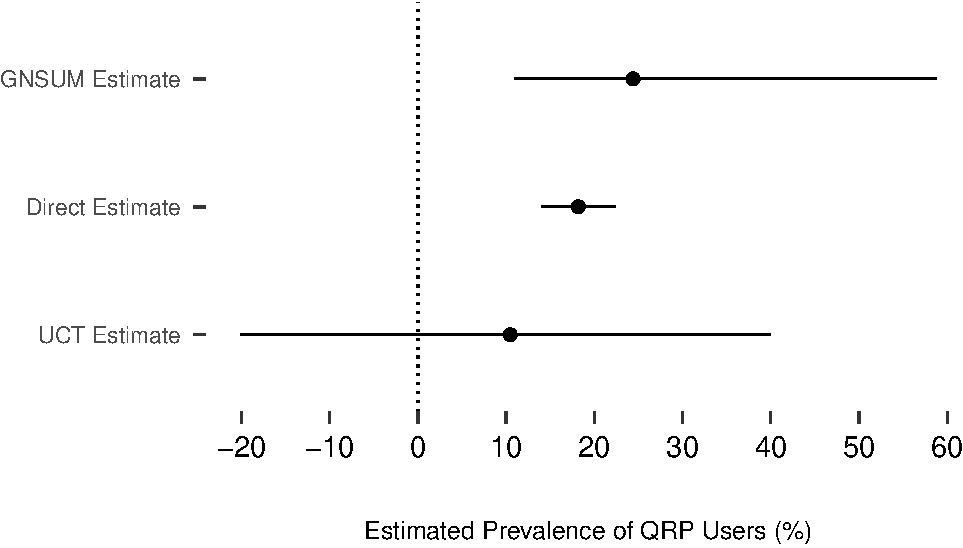
\includegraphics{papaja_output_files/figure-latex/unnamed-chunk-12-1.pdf}
\caption{\label{fig:unnamed-chunk-12}\label{fig:fig1}Estimates of the
current prevalence of users of questionable research practices using
three different estimators; the Generalized Network Scale-Up Method
(GNSUM), the Direct Estimate, and the Unmatched Count Technique (UCT).
Point estimates with 95\% bootstrapped confidence intervals.}
\end{figure}

\subsection{Direct Estimate}\label{direct-estimate-1}

To ensure the highest number of participants in our game of contacts,
half of the total population were asked to participate in Survey 3,
which contained our direct estimate question. Thus, 3,551 psychologists
were solicited, and we received 308 responses to Survey 3 able to be
analyzed. Of the 308 participants, 56 indicated they had used at least
one QRP in the past 12 months. Using Equation 1, we calculated QRP
prevalence to be 18.18\% (bootstrapped 95\% confidence interval
{[}13.96\%, 22.40\%{]}). This corresponds to an estimated 1291 American
psychologists currently using QRPs.

It is possible this estimate is underestimating the true number of
psychologists using QRPs. For one, social desirability may influence QRP
users to conceal their identity when asked directly. In that case, our
estimate is only generated by those participants willing to reveal their
identity. Given the somewhat critical social environment for QRP users
(Fiske, 2016), it is reasonable to believe some participants withheld
their identity when we asked directly. The following indirect estimation
methods sought to mitigate this social desirability bias.

\subsection{Unmatched Count
Technique}\label{unmatched-count-technique-1}

The remaining 3,550 psychologists contacted were asked to participate in
our unmatched count estimate with 1,775 randomized into the innocuous
list condition, and 1,775 randomized into the sensitive list condition.

The average number of list items corresponding to participants in the
innocuous list condition was 4.28. The average number of list items
corresponding to participants in the sensitive list condition was 4.39.
Using Equation 2, we calculated QRP user prevalence to be 10.46\%
{[}-20.19\%, 22.40\%{]}. This corresponds to an estimated 743 American
psychologists currently using QRPs.

It was unexpected that an UCT estimate lower than our direct estimate
would be calculated. Typically, due to reducing response bias, UCT
estimates tend to be larger than direct estimates when the behavior or
identity in question is stigmatized (Gervais \& Najle, 2017; Starosta \&
Earleywine, 2014; Wolter \& Laier, 2014). The fact that the bootstrapped
confidence interval crosses zero indicates instibility in the sensitive
list being consistantly larger than the control list. It is likely our
relatively low number of participants in our UCT estimate (n = 279) led
this calculation to be overly sensitive to individual responses. This is
not the first time the UCT has provided smaller estimates than a direct
estimate (Arentoft et al., 2016), though given the high variability, we
do not have confidence that this UCT estimate is a valid estimate of
current QRP use.

\subsection{Generalized Network Scale-Up
Estimate}\label{generalized-network-scale-up-estimate}

All participants who were randomized into the UCT estimate were also
asked to answer questions about their social networks, and to estimate
how many researchers they know who have used at least one QRP in the
past 12 months. Participants who were randomized into the direct
estimate and who self-identified as a QRP user in that estimate were
also asked to answer questions about their social network and to
participate in the game of contacts method. Participants in the direct
estimate who did not self-identify as a QRP user were asked questions
about their social network as well, but were not asked how many
researchers they know who have used at least one QRP in the past 12
months. Therefore, we collected social network responses from 531
participants from the general frame population (to be used in estimating
\(\delta\)), 56 responses from participants who self-identified as QRP
users who also completed the game of contacts (to be used in estimating
\(\tau\)), and 279 responses from participants who estimated the number
of researchers they know who have used at least one QRP in the past 12
months.

These 279 identified 664 QRP users, and know a collective 46,828
researchers. Given the total frame population is 7,101, we are fairly
confident all members were identified at least once by our participants.
Using the network scale-up in Equation 3, this generates an estimate of
1.42\% {[}0.85\%, 2.14\%{]}. This estimate serves as the base starting
point for Equation 4, the Generalized Network Scale-Up Estimator,
detailed below.

Equation 4 relaxes the assumptions of equal network size and total
information transmission by incorporating \(\tau\) and \(\delta\). Using
the 531 responses from the general population, plus the 56 responses
from the participants who indicated using a QRP in the past 12 months,
we estimate \(\delta\) as . Using the game of contacts, we estimate
\(\tau\) as 0.06. Using Equation 4, we estimate QRP user prevalence to
be 24.40\% {[}10.93\%, 58.74\%{]}. This corresponds to an estimated 1733
American psychologists currently using QRPs.

To assess the accuracy of participants in estimating the size of this
unknown group (QRP users), we asked questions about 24 populations of
known size (number of researchers named David, named Janet, etc). The 24
names were gender balanced and represented common, uncommon, and rare
names that exist within the census of the frame population. The size
estimates of these populations of known size can be seen in Figure 2.
These estimates seem reasonable and closely mirror the actual prevalence
of these groups. The fact that the same estimator in the same group of
participants can generate reasonable estimates for populations of known
size is encouraging evidence of the accuracy of our estimate of the
number of recent QRP users utilizing the generalized network scale-up
estimate.

\begin{figure}
\centering
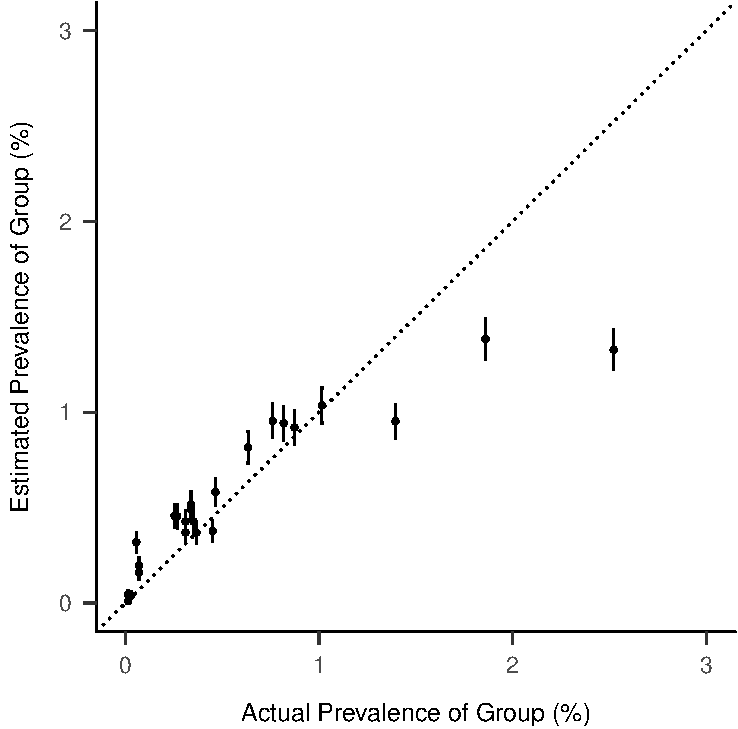
\includegraphics{papaja_output_files/figure-latex/unnamed-chunk-14-1.pdf}
\caption{\label{fig:unnamed-chunk-14}\label{fig:fig2}Validation of Network
Scale-Up Estimates using 24 groups of known size. Each point represents
one group, with 95\% confidence intervals. Dotted line represents when
estimated group size equals actual group size.}
\end{figure}

\section{DISCUSSION}\label{discussion}

To the best of our knowledge, this is the first report of the prevalence
of QRPs in a proximal timespan. As such, it is difficult to draw
conclusions about the magnitude of our estimates when compared to
previous estimates. Compared to John et al. (2012) and Agnoli et al.
(2017), we estimate lower rates of questionable research practices.
Compared to Fiedler and Schwarz (2016), however, we estimate higher
rates of these practices. Our definition of \enquote{questionable
research practices} were the same ones used in John et al. (2012) and
Agnoli et al. (2017), but was restricted to a timespan of only 15
months, so it is reasonable that our estimates would be lower than those
with an unrestricted time of QRP use. Since we used those same QRP
definitions, is also reasonable that our estimates would be higher than
those described by Fiedler and Schwarz (2016), who changed the
definition of each QRP. We also measured true \enquote{prevalence}, that
is, the commonality of a behavior within a designated time frame, which
was a point of difference between John et al. (2012) and Fiedler and
Schwarz (2016).

This is also the first report to use the network scale-up and
generalized network-scale up estimators to investigate the ongoing
reproducibility issues in psychology. Re-framing QRP prevalence away
from the individual behavior and towards the user state brings our
field-wide problems more into scope with existing literature on stigma
and concealable identities. For example, much work has been done
focusing on how increasing stigma inadvertently locks individuals into
detrimental behaviors (Stuber, Galea, \& Link, 2009), and how revealing
a concealed identity can increase well-being by reducing the stress of
being exposed (Chaudoir \& Quinn, 2010). Framing QRP use in terms of the
individual may help the field reduce QRP use by increasing awareness of
the effects of stigma and support.

\subsection{Implications}\label{implications}

These estimates serve as a baseline to measure the effectiveness of
current initiatives, as well as a foundation for new ones. While much
work is being done to grow support for interventions such as
pre-registration (CITATION) and Registered Reports (CITATION), it is
currently unknown what quantitative effect these are having on curbing
behaviors associated with inflated Type I error such as QRPs. By
performing follow-up estimates, the field can use these baseline
estimates to measure the effectiveness of these programs and make
informed decisions on their effectiveness.

\subsection{Limitations \& Future
Directions}\label{limitations-future-directions}

Our unmatched count estimate produced a value with a confidence interval
that crossed zero, meaning there was sufficient variance to destabilize
the group difference we observed. As mentioned previously, the
relatively low number of participants for the unmatched count estimate
() contributed to this high variability. Future work using the unmatched
count technique would benefit from larger sample sizes (as demonstrated
in Gervais and Najle (2017), which used 2000 participants).

These estimates were limited to American psychologists, though we know
that these issues are not contained solely in the United States (Stapel
CITATION). Future studies estimating the prevalence of QRPs in other
countries will be an important next step. Some of this work has already
started through the Horizon 2020 framework in the European Union
(PRINTEGER CITATION), though more innovative work will be required to
better understand the scope of the problems faced by our field.

\subsection{Conclusion}\label{conclusion}

By directly asking participants about their use of QRPs, we estimate
18.18\% have used at least one QRP in the past 12 months, and the
generalized network scale up estimate is 24.40\%, which corresponds to
between 1291 and 101 American psychologists. While some argue the
narrative of the \enquote{replication crisis} is overblown (Fanelli,
2018), the current work illustrates how common these behaviors that
inflate false-positive findingss are. Although many have called for
changes in statistical inference practices to mitigate false-positive
findings (Benjamin et al., 2017; Lakens et al., 2018), it is important
that we as a field continue to focus on disincentivizing the use of
questionable research practices (and other behavioral degrees of
freedom) among our peers and coworkers for the betterment of our
science.

\newpage

\section{References}\label{references}

\begingroup
\setlength{\parindent}{-0.5in} \setlength{\leftskip}{0.5in}

\hypertarget{refs}{}
\hypertarget{ref-Agnoli2017}{}
Agnoli, F., Wicherts, J. M., Veldkamp, C. L. S., Albiero, P., \&
Cubelli, R. (2017). Questionable research practices among Italian
research psychologists. \emph{PLoS ONE}, \emph{12}(3), 1--17.
doi:\href{https://doi.org/10.1371/journal.pone.0172792}{10.1371/journal.pone.0172792}

\hypertarget{ref-Arentoft2016}{}
Arentoft, A., Van Dyk, K., Thames, A. D., Sayegh, P., Thaler, N.,
Schonfeld, D., \ldots{} Hinkin, C. H. (2016). Comparing the unmatched
count technique and direct self-report for sensitive health-risk
behaviors in HIV+ adults. \emph{AIDS Care - Psychological and
Socio-Medical Aspects of AIDS/HIV}, \emph{28}(3), 370--375.
doi:\href{https://doi.org/10.1080/09540121.2015.1090538}{10.1080/09540121.2015.1090538}

\hypertarget{ref-Banks2016}{}
Banks, G. C., O'Boyle, E. H., Pollack, J. M., White, C. D., Batchelor,
J. H., Whelpley, C. E., \ldots{} Adkins, C. L. (2016). Questions About
Questionable Research Practices in the Field of Management: A Guest
Commentary. \emph{Journal of Management}, \emph{42}(1), 5--20.
doi:\href{https://doi.org/10.1177/0149206315619011}{10.1177/0149206315619011}

\hypertarget{ref-Benjamin2017}{}
Benjamin, D. J., Berger, J. O., Johannesson, M., Nosek, B. A.,
Wagenmakers, E. J., Berk, R., \& Johnson, V. E. (2017). Redefine
Statistical Significance. \emph{PsyArxiv}, (July 22), 1--18.
doi:\href{https://doi.org/10.17605/OSF.IO/MKY9J}{10.17605/OSF.IO/MKY9J}

\hypertarget{ref-Bernard2010}{}
Bernard, H. R., Hallett, T., Iovita, A., Johnsen, E. C., Lyerla, R.,
McCarty, C., \ldots{} Stroup, D. F. (2010). Counting hard-to-count
populations: the network scale-up method for public health.
\emph{Sexually Transmitted Infections}, \emph{86 Suppl 2}, ii11--5.
doi:\href{https://doi.org/10.1136/sti.2010.044446}{10.1136/sti.2010.044446}

\hypertarget{ref-Button2013}{}
Button, K. S., Ioannidis, J. P. A., Mokrysz, C., Nosek, B. A., Flint,
J., Robinson, E. S. J., \& Munafò, M. R. (2013). Power failure: why
small sample size undermines the reliability of neuroscience.
\emph{Nature Reviews Neuroscience}, \emph{14}(5), 365--376.
doi:\href{https://doi.org/10.1038/nrn3475}{10.1038/nrn3475}

\hypertarget{ref-Chaudoir2010}{}
Chaudoir, S. R., \& Quinn, D. M. (2010). Revealing Concealable
Stigmatized Identities: The Impact of Disclosure Motivations and
Positive First-Disclosure Experiences on Fear of Disclosure and
Well-Being. \emph{Journal of Social Issues}, \emph{66}(3), 570--584.
doi:\href{https://doi.org/10.1111/j.1540-4560.2010.01663.x}{10.1111/j.1540-4560.2010.01663.x}

\hypertarget{ref-Fanelli2009a}{}
Fanelli, D. (2009). How many scientists fabricate and falsify research?
A systematic review and meta-analysis of survey data. \emph{PLoS ONE},
\emph{4}(5).
doi:\href{https://doi.org/10.1371/journal.pone.0005738}{10.1371/journal.pone.0005738}

\hypertarget{ref-Fanelli2018}{}
Fanelli, D. (2018). Is science really facing a reproducibility crisis,
and do we need it to? \emph{Proceedings of the National Academy of
Sciences of the United States of America2}, \emph{in press}, 1--4.
doi:\href{https://doi.org/10.1073/pnas.1708272114}{10.1073/pnas.1708272114}

\hypertarget{ref-Fiedler2016}{}
Fiedler, K., \& Schwarz, N. (2016). Questionable Research Practices
Revisited. \emph{Social Psychological and Personality Science},
\emph{7}(1), 45--52.
doi:\href{https://doi.org/10.1177/1948550615612150}{10.1177/1948550615612150}

\hypertarget{ref-Fiske2016}{}
Fiske, S. T. (2016). Mob Rule or Wisdom of Crowds. \emph{APS Observer}.

\hypertarget{ref-Gervais2017}{}
Gervais, W. M., \& Najle, M. B. (2017). How many atheists are there?
\emph{Social Psychological and Personality Science}, 1948550617707015.

\hypertarget{ref-Jing2014}{}
Jing, L., Qu, C., Yu, H., Wang, T., \& Cui, Y. (2014). Estimating the
sizes of populations at high risk for HIV: A comparison study.
\emph{PLoS ONE}, \emph{9}(4), 1--6.
doi:\href{https://doi.org/10.1371/journal.pone.0095601}{10.1371/journal.pone.0095601}

\hypertarget{ref-John2012}{}
John, L. K., Loewenstein, G., \& Prelec, D. (2012). Measuring the
Prevalence of Questionable Research Practices With Incentives for Truth
Telling. \emph{Psychological Science}, \emph{23}(5), 524--532.
doi:\href{https://doi.org/10.1177/0956797611430953}{10.1177/0956797611430953}

\hypertarget{ref-Lakensabc1860}{}
Lakens, D., Adolfi, F. G., Albers, C. J., Anvari, F., J Apps, M. A.,
Argamon, S. E., \ldots{} Lino de Oliveira, C. (2018). Justify Your
Alpha: A Response to `` Redefine Statistical Significance''.
\emph{Nature Human Behavior}, \emph{2}, 168--171.

\hypertarget{ref-Lu2009}{}
Lu, Y.-E., Roberts, S., Lio, P., Dunbar, R., \& Crowcroft, J. (2009).
Size Matters: Variation in Personal Network Size, Personality and Effect
on Information Transmission. \emph{2009 International Conference on
Computational Science and Engineering}, (217141), 188--193.
doi:\href{https://doi.org/10.1109/CSE.2009.179}{10.1109/CSE.2009.179}

\hypertarget{ref-Salganik2011}{}
Salganik, M. J., Fazito, D., Bertoni, N., Abdo, A. H., Mello, M. B., \&
Bastos, F. I. (2011). Assessing network scale-up estimates for groups
most at risk of HIV/AIDS: Evidence from a multiple-method study of heavy
drug users in Curitiba, Brazil. \emph{American Journal of Epidemiology},
\emph{174}(10), 1190--1196.
doi:\href{https://doi.org/10.1093/aje/kwr246}{10.1093/aje/kwr246}

\hypertarget{ref-Simmons2011}{}
Simmons, J. P., Nelson, L. D., \& Simonsohn, U. (2011). False-Positive
Psychology. \emph{Psychological Science}, \emph{22}(11), 1359--1366.
doi:\href{https://doi.org/10.1177/0956797611417632}{10.1177/0956797611417632}

\hypertarget{ref-Starosta2014}{}
Starosta, A. J., \& Earleywine, M. (2014). Assessing base rates of
sexual behavior using the unmatched count technique. \emph{Health
Psychology and Behavioral Medicine}, \emph{2}(1), 198--210.
doi:\href{https://doi.org/10.1080/21642850.2014.886957}{10.1080/21642850.2014.886957}

\hypertarget{ref-Stuber2009}{}
Stuber, J., Galea, S., \& Link, B. G. (2009). Stigma and Smoking: The
Consequences of Our Good Intentions. \emph{Social Service Review},
\emph{83}(4), 585--609.
doi:\href{https://doi.org/10.1086/650349}{10.1086/650349}

\hypertarget{ref-Tukey1970}{}
Tukey, J. W. (1970). \emph{Exploratory Data Analysis}.

\hypertarget{ref-Wicherts2016}{}
Wicherts, J. M., Veldkamp, C. L., Augusteijn, H. E., Bakker, M., Aert,
R. C. van, \& Assen, M. A. van. (2016). Degrees of freedom in planning,
running, analyzing, and reporting psychological studies: A checklist to
avoid P-hacking. \emph{Frontiers in Psychology}, \emph{7}(NOV), 1--12.
doi:\href{https://doi.org/10.3389/fpsyg.2016.01832}{10.3389/fpsyg.2016.01832}

\hypertarget{ref-Wolter2014}{}
Wolter, F., \& Laier, B. (2014). The Effectiveness of the Item Count
Technique in Eliciting Valid Answers to Sensitive Questions. An
Evaluation in the Context of Self-Reported Delinquency. \emph{Survey
Research Methods}, \emph{8}(3), 153--168.

\hypertarget{ref-Zhang2010}{}
Zhang, T. Y., Hellstrom, I. C., Bagot, R. C., Wen, X., Diorio, J., \&
Meaney, M. J. (2010). Maternal care and DNA methylation of a glutamic
acid decarboxylase 1 promoter in rat hippocampus. \emph{J Neurosci},
\emph{30}(39), 13130--13137.
doi:\href{https://doi.org/10.1523/JNEUROSCI.1039-10.2010}{10.1523/JNEUROSCI.1039-10.2010}

\hypertarget{ref-Zheng2006}{}
Zheng, T., Salganik, M. J., \& Gelman, A. (2006). How Many People Do You
Know in Prison? \emph{Journal of the American Statistical Association},
\emph{101}(474), 409--423.
doi:\href{https://doi.org/10.1198/016214505000001168}{10.1198/016214505000001168}

\endgroup


\end{document}
